\documentclass[
  letterpaper, % page size
  fontsize=10pt, % base font size
  twoside=true,
  chapterentrydots=true, % in the TOC, puts dots between name and page number
  numbers=noenddot,
  fontmethod=tex,
]{kaobook}

\usepackage[english]{babel}
\usepackage[english=british]{csquotes}

% \usepackage{kaobiblio}
% \addbibresource{handbook.bib}

\usepackage[framed=true]{kaotheorems}

\usepackage{kaorefs}

\usepackage{makecell}

\usepackage{lib/kaoref-extended}
\usepackage{lib/regulation}
\usepackage{lib/pbp-ref}

\graphicspath{{images/}}
%\graphicspath{{deep/path/images/}{images/}}

\makeindex[columns=3,title=Alphabetical Index,intoc]

% \makeglossaries
% \newglossaryentry{computer}{
	name=computer,
	description={is a programmable machine that receives input, stores and manipulates data, and provides output in a useful format}
}

% Glossary entries (used in text with e.g. \acrfull{fpsLabel} or \acrshort{fpsLabel})
\newacronym[longplural={Frames per Second}]{fpsLabel}{FPS}{Frame per Second}
\newacronym[longplural={Tables of Contents}]{tocLabel}{TOC}{Table of Contents}



\makenomenclature

% Reset sidenote counter at chapters
%\counterwithin*{sidenote}{chapter}

\begin{document}

% \titlehead{Displayed Top-Left on title page}
% \subject{Displayed under title}

\title[ECCC Race Handbook]{
  Collegiate Race Handbook \\
  Eastern Collegiate Cycling Conference
}
\subtitle{A comprehensive guide}

\author{Flyyn Leonard}
\date{\today}

\publishers{Northeast Collegiate Cycling Corporation}


\frontmatter

% TODO: opening page
% TODO: copyright page

\maketitle

% TODO: preface

% -------------------------------------------
% Table of Contents & Lists of Figures/Tables
% -------------------------------------------

\begingroup
\setlength{\textheight}{230\hscale} % Manually adjust height of TOC pages

% Turn on compatibility mode for etoc package
\etocstandarddisplaystyle
\etocstandardlines

\tableofcontents

\listofregulations

\listoffigures

% \listoftables

% \listoflstlistings

\endgroup

\mainmatter
\setchapterstyle{kao}

\pagelayout{wide}
\addpart{Introduction}
\pagelayout{margin}

% TODO: image is stretched, fix
\setchapterimage[7cm]{IMG_7884.jpg}
\setchapterpreamble[u]{\margintoc}
\chapter{Road Race Play-By-Play}
\labch{road-play-by-play}

This chapter will walk through the brainstorming,
planning, setup, execution, and post-event paperwork and tasks for a hypothetical collegiate road race weekend.%
\footnote{For a similar play-by-play description of a mountain race weekend,
see \nrefch{mtb-play-by-play}}

This chapter attempts to be generic, and should be applicable for both
\nfirstrefsec{hosting:conference} and
\nfirstrefsec{hosting:team}.

\section{Assembling a Team}

A race weekend takes a large amount of work, and is near impossible for one person to handle alone.
However, planning and running the weekend can be simple if you have the right team to delegate work to.

Each race may divide responsibilities differently, especially if events are run by the conference
vs. being student run, but this play-by-play will describe work using a standard set of roles.

\subsubsection{Race Lead Organizer}

The \pbproleref{role:lead_org}%
\sidenote{%
  See \pgrefsubsec{role:lead_org} for a list of duties and responsibilities for this role.
}
is the first role that should be assigned.
This person must be part of the organization legally/financially hosting the race, and will be tasked with ensuring the success of the race
from start to finish.

For \nameref{sec:hosting:conference}, % TODO: better reference format
this will be the \pbproleref{role:eccc_season_coordinator}%
\sidenote{%
  See \frefsec{role:eccc_coordination_team} for information about the season coordinators,
  including the current season coordinators for each discipline.%
}.
For \nameref{sec:hosting:team},
this is typically a team member in a leadership position.

\section{Planning and Paperwork}

\index{mapping software!Trailforks}
The \pbproleref{role:race_org_team} should prepare a few potential routes for each event,
typically using software like Trailforks or MapMyRide as shown in \reffig{road_pbp_trailforks}.

\pbproleref{role:local_teams} can assist the primary organizing organization with their local knowledge of roads and venues.

\begin{figure}[h]
  \includegraphics[width=1\textwidth]{2024_groton_trailforks.png}
  \caption[Road race course map in Trailforks]{
    A potential road race course in Groton, MA
    prepared via Trailforks for the 2024 Road Season.\\
    Credit: Flyyn Leonard}
  \labfig{road_pbp_trailforks}
\end{figure}


The \pbproleref{role:lead_org} should contact the local town or city
to determine what permits may be required, and make an initial contact to the police department,
as the police are typically a critical component to planning and running the race.

Once the race has passed the initial hurdle of getting a route and hasn't been shot down by the local government,
the \pbproleref{role:race_org_team} should evaluate local services and get quotes for:

\begin{itemize}
  \item Medical coverage, often by a local fire department or contracted private ambulance service
  \item Barriers and other course supplies - these may be supplied by the local police or highway department, or rented from private companies
  \item Additional venues for parking and staging (described in more detail below)
\end{itemize}

The \pbproleref{role:eccc_coordination_team} is available to help and advise the organizing team throughout this entire process,
and can often provide suggestions of who to contact, and have a list of departments and private companies that have been used in the past.

\subsubsection{Additional Venues}

Along with the on-road courses, you will need to plan where riders will park,
an area where an intro-clinic can be held (for criterium days),
a place to setup registration,
a finish line,
and an area by the course for staging.

These locations may all be in one large parking lot, or multiple smaller venues can be used.

Many ECCC races have had good luck contacting local K-12 schools, which are typically available for the weekend.

\subsection{Budget}

Using all of the information gathered in the initial planning phase, the \pbproleref{role:race_org_team} should start drafting a race budget
to ensure the race will be financially viable.

This budget can also serve as a to-do list, reminding organizers of the various services that will need to be contracted for the event.

A sample budget is included in \nrefch{event_budget}, and teams can contact the \pbproleref{role:eccc_coordination_team}
for a digital copy of the ECCC race budget template.
Using the official ECCC budget format is preferred, allowing ECCC staff to easily compile and compare budgets across weekends and years.

Teams should contact the \pbproleref{role:eccc_coordination_team} to discuss what registration fees should be for the entire season -
the ECCC tries to keep registration fees consistent across all races of the season, which makes it easy for teams to register.

\subsection{Flyer Design}

\begin{marginfigure}
  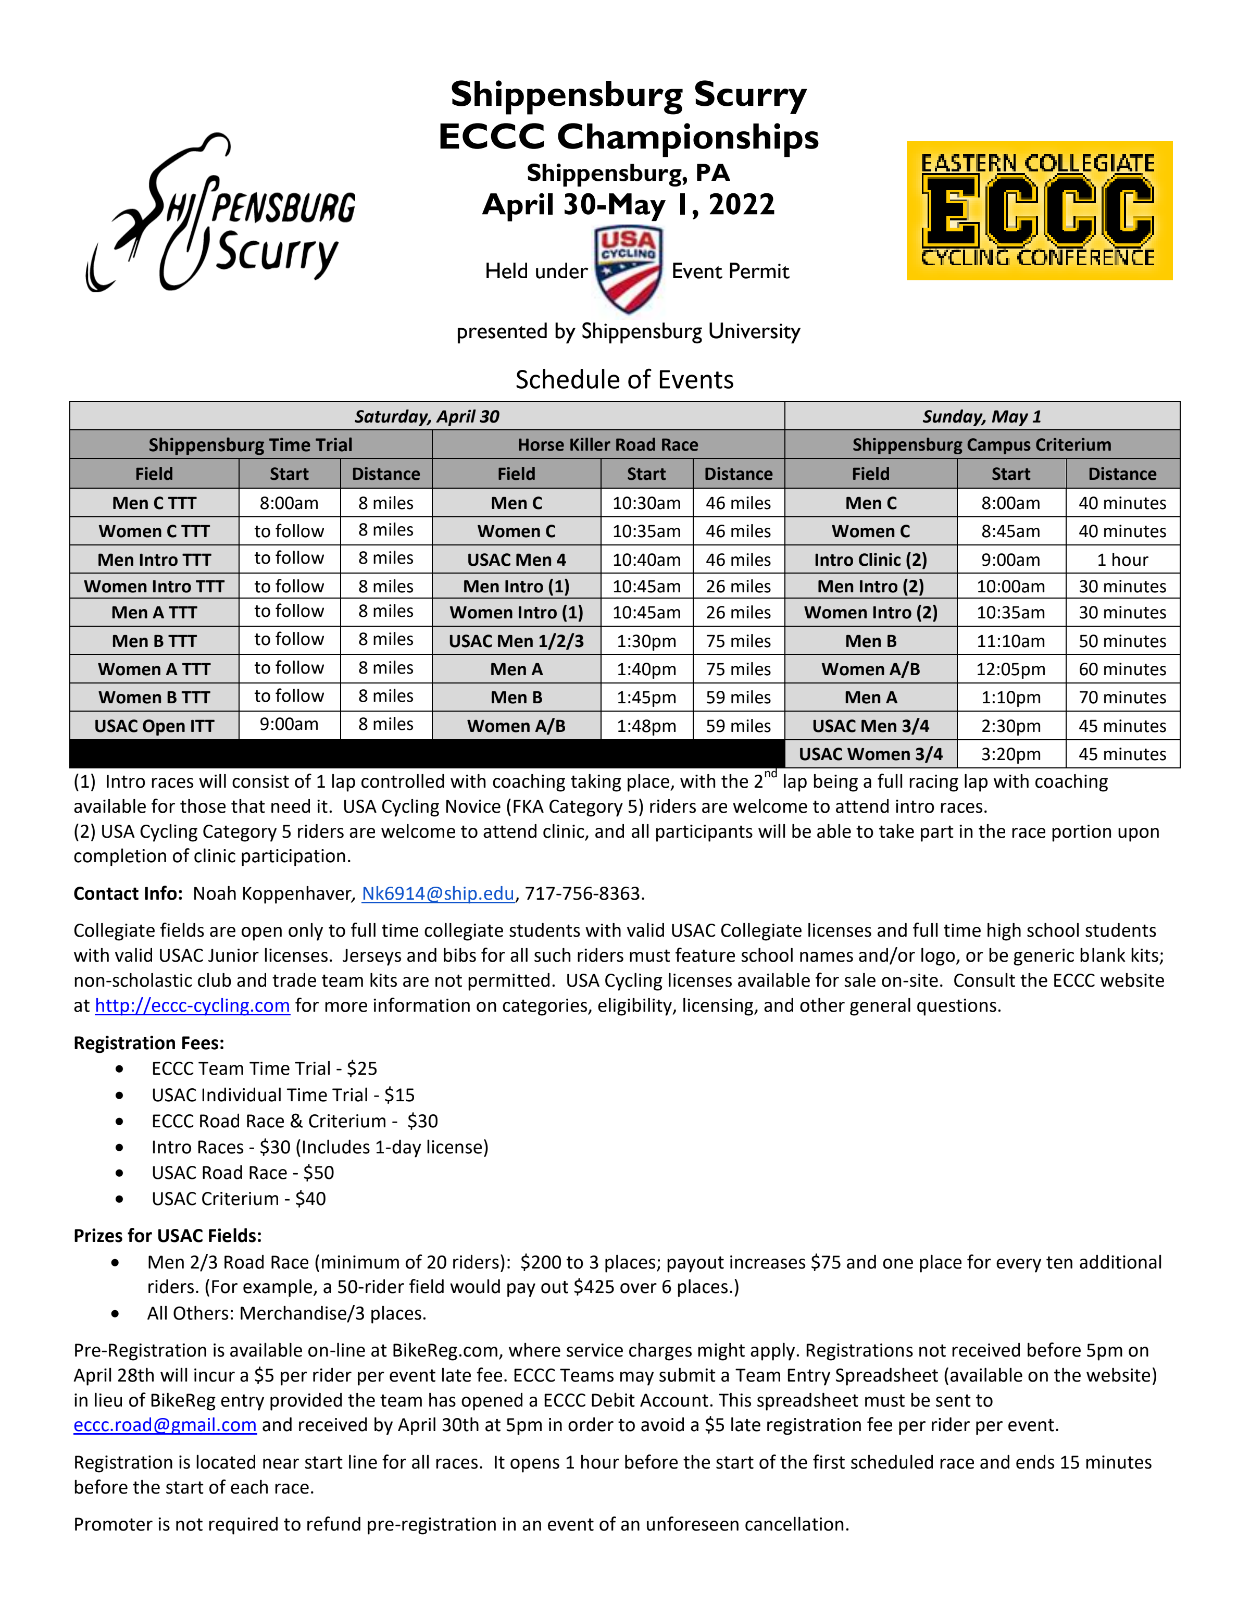
\includegraphics{2022_ship_scurry_flyer_pg1.png}
  \caption[An example race flyer]{A race flyer with the standard USA Cycling/ECCC formatted event schedule, from the 2022 Shipensburg Scurry}
  \labfig{road_pbp_flyer}
\end{marginfigure}

Once the race is deemed viable, the \pbproleref{role:race_org_team} should prepare a flyer, working with the \pbproleref{role:eccc_coordination_team}
to ensure the flyer meets the standard format dictated by the USA Cycling permitting process as well as the ECCC standards.

Race flyers should include:
\begin{itemize}
  \item The event schedule (in a USA Cycling approved format)
  \item Course maps for each event
  \item The address(es) of the race venue(s)
  \item The registration fees (noting day-of surcharges and student discounts)
  \item The methods of registration, including online (BikeReg), collegiate team bulk registration, and in-person day-of registration
  \item The deadlines for registering
  \item Driving directions (and other forms of transportation if applicable, such as public transportation)
  \item The type and format of contracted medical standby services, and the address of the nearest hospital for each venue
\end{itemize}

The race flyer is critical to obtaining a USA Cycling event permit.

\subsection[USA Cycling Permitting]{Obtaining a USA Cycling Permit}

Working with the \pbproleref{role:eccc_coordination_team}, the \pbproleref{role:lead_org} should submit a USA Cycling event permit application.

Once approved, this will provide Certificates of Insurance (COI) % TODO: add to glossary
that are typically required by the local government and venues,
and should automatically start the process of getting USA Cycling Officials to work the event.

\begin{marginfigure}
  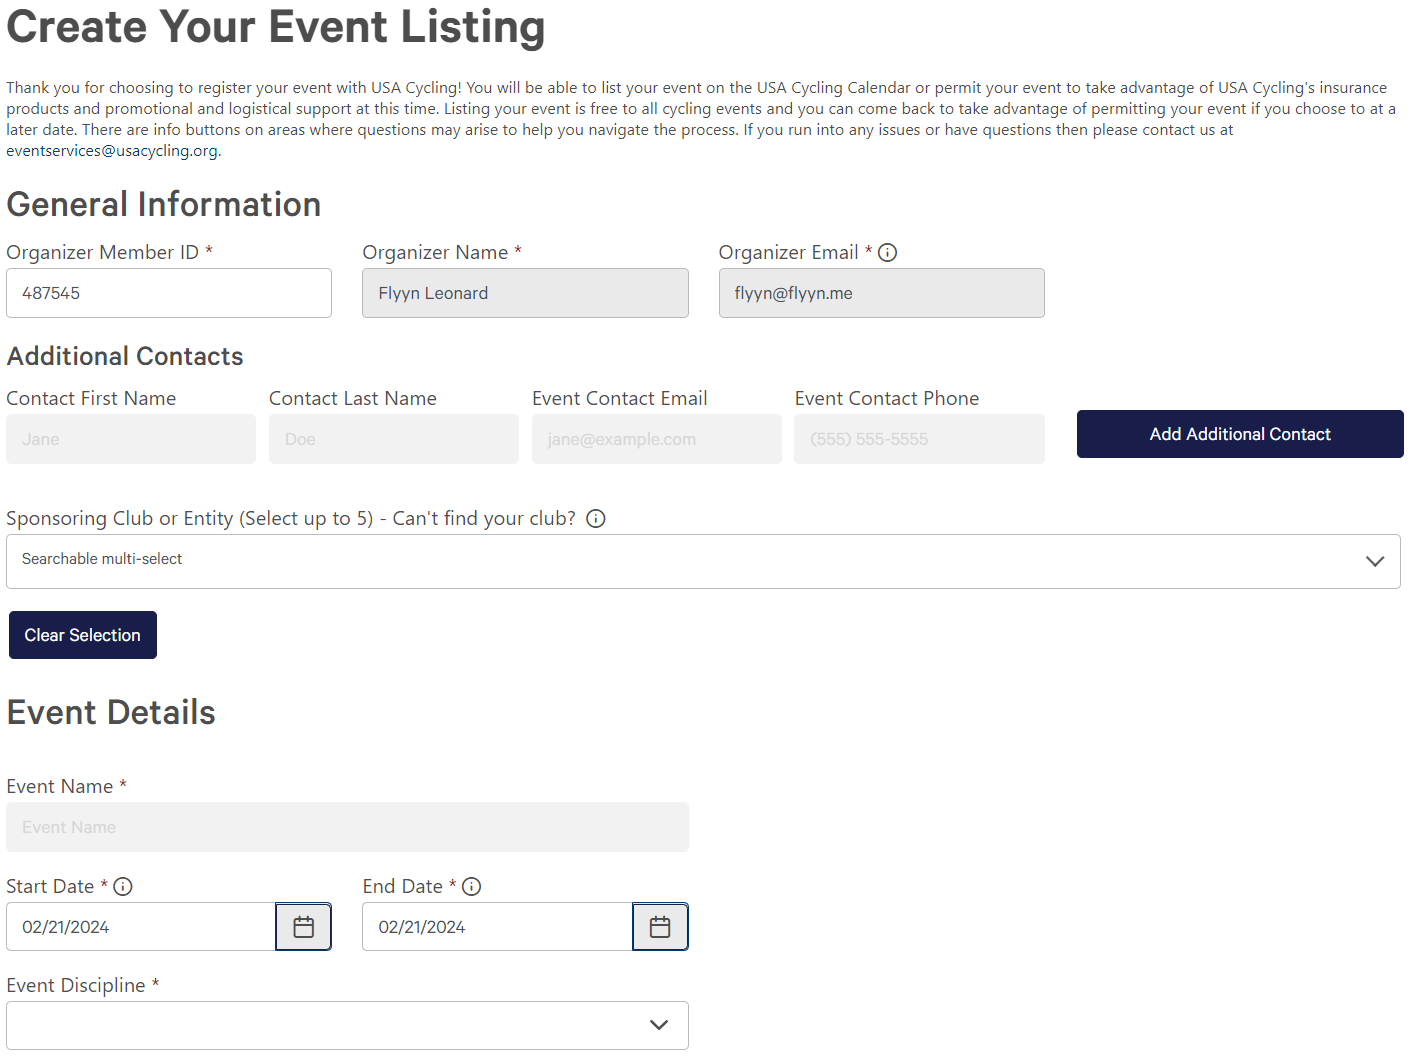
\includegraphics{2024_usac_permit_application.png}
  \caption{USA Cycling event permit application form}
  \labfig{road_pbp_usac_permit_app}
\end{marginfigure}

\subsection{Additional Planning}

Along with all the essential items above, there's additional items that need to be coordinated.

\subsubsection{Marketing and Sponsorship}

The current collegiate turnout to a race weekend will likely not generate enough registration funds to balance your budget.
Most ECCC races use two key elements to balance the budget: advertising race fields for non-collegiate riders, and getting sponsorship.

The \pbproleref{role:lead_org} should consider the existing connections to sponsors that they may be able to request event-specific sponsorship from,
and should also evaluate if there are local businesses, such as bike shops or banks that might sponsor the event.

\pbproleref{role:local_teams} can be a huge assistance finding local media and other marketing opportunities, and could contact their team sponsors
in case the sponsors might be interested in sponsoring the event.

\subsubsection{Online Registration}

The \pbproleref{role:eccc_season_coordinator} will work with the \pbproleref{role:lead_org} to setup BikeReg pages for the event,
traditionally using the ECCC's BikeReg account.

\subsubsection{Volunteer Signup}

The \pbproleref{role:primary_promoter} should work with the \pbproleref{role:assistant_promoter} to ensure that all volunteer positions will be filled,
including lead/follow cars and drivers, and course marshalling.

Typically the promoters will reach out to \pbproleref{role:local_teams} to find volunteers.

\subsubsection{Food Planning}

The ECCC expects that the \pbproleref{role:lead_org} will plan to feed the officials, medical staff, and the \pbproleref{role:race_ops_team}.
% TODO: document this expectation as a regulation (in the rules section), and link to the regulation
Additionally, races typically provide some food for marshals as a thank-you (often in the form of pizza).

\section{Course Preparation}

In the months, weeks, and days leading up to the race, some on-site work may need to be done.

According to USA Cycling regulations, the \pbproleref{role:chief_ref} may request to preview the course well before the race.
This allows the \pbproleref{role:chief_ref} to assess the safety and design of the event.

Regardless of the official's preview, the \pbproleref{role:lead_org} should ensure that someone previews the course 5-7 days before the event.
This preview should check:
\begin{itemize}
  \item The state of potholes, sewer grates, and other hazards that may need to be mitigated
  \item The presence of any construction, detours, or other obstacles that may require changes to the course
  \item A final review of where marshals may be needed, and where the finish line should be located
\end{itemize}

\subsubsection{Signage and Notifying Residents}

The \pbproleref{role:lead_org} should coordinate with the local police and find out how local residents should be notified of the race.

Often the \pbproleref{role:race_org_team} will need to drop off a letter at each residence (working with \pbproleref{role:local_teams} if needed),
but sometimes the police will suggest using social media or reverse 911 to contact residents.

Additionally, the \pbproleref{role:lead_org} should check if no-parking signs can be put up.
Often the no-parking signs should be put up the night before the race, or one day in advance.

% TODO: any legal notes?

The \pbproleref{role:lead_org} should consider other local signage, such as advertising signs that could be put up in the town,
or signs directing arriving participants to the venue.

\subsubsection{Barriers}

Well before the race, the \pbproleref{role:lead_org} should coordinate with the local police and/or highway department
to ensure that barriers can be placed around the race course.
For a criterium, often the entire course is shut down with barriers, police officers, and marshals.
With a road race course, barriers are less often used (as the entire course is typically open to traffic), but barriers can be used
as ``checkpoints'' to control the traffic flow as cars approach the course.

In some cases, the police or highway department will require that they setup the barriers themselves (often at an additional cost),
as road closures are an official matter.

Other times, the police will ask the \pbproleref{role:lead_org} to move barriers the night before the race,
so the detail officers just need to move the barriers into position when they arrive on the day of the event.

\section{Race Weekend}

It's now the night before the first race - hopefully all the planning and preparations listed above are complete!

This section will chronologically walk through a hypothetical race weekend from Friday night before the first race,
through the end of the last race on Sunday afternoon.

For this example, there will be a criterium on Saturday,
and a team time trial (TTT) % TODO: put in glossary
and road race held on Sunday.

You will notice that roles shift as we transition from planning to the weekend operations -
in the previous planning sections, the \pbproleref{role:lead_org} was tasked with most work.
During the weekend, the \pbproleref{role:primary_promoter} will take the primary responsibility for the event.

A few example emergencies are included in this section, based on actual emergencies that have happened at previous ECCC races
(with some details changed for anonymity).
While we've attempted to include some unusual cases, keep in mind that emergencies may happen at any time, and can be highly unique and unusual.

\subsection{Friday Preparation}

The day before the criterium, the \pbproleref{role:lead_org} should ensure the crit course is swept and otherwise cleaned up,
either themselves or with assistance from \pbproleref{role:local_teams}.

Any no-parking signs, barriers, or other materials should be deployed (following the guidance and regulations of the local police and highway department).

The \pbproleref{role:lead_org} should have contracted a towing company to clear the crit course overnight.

\begin{marginfigure}
  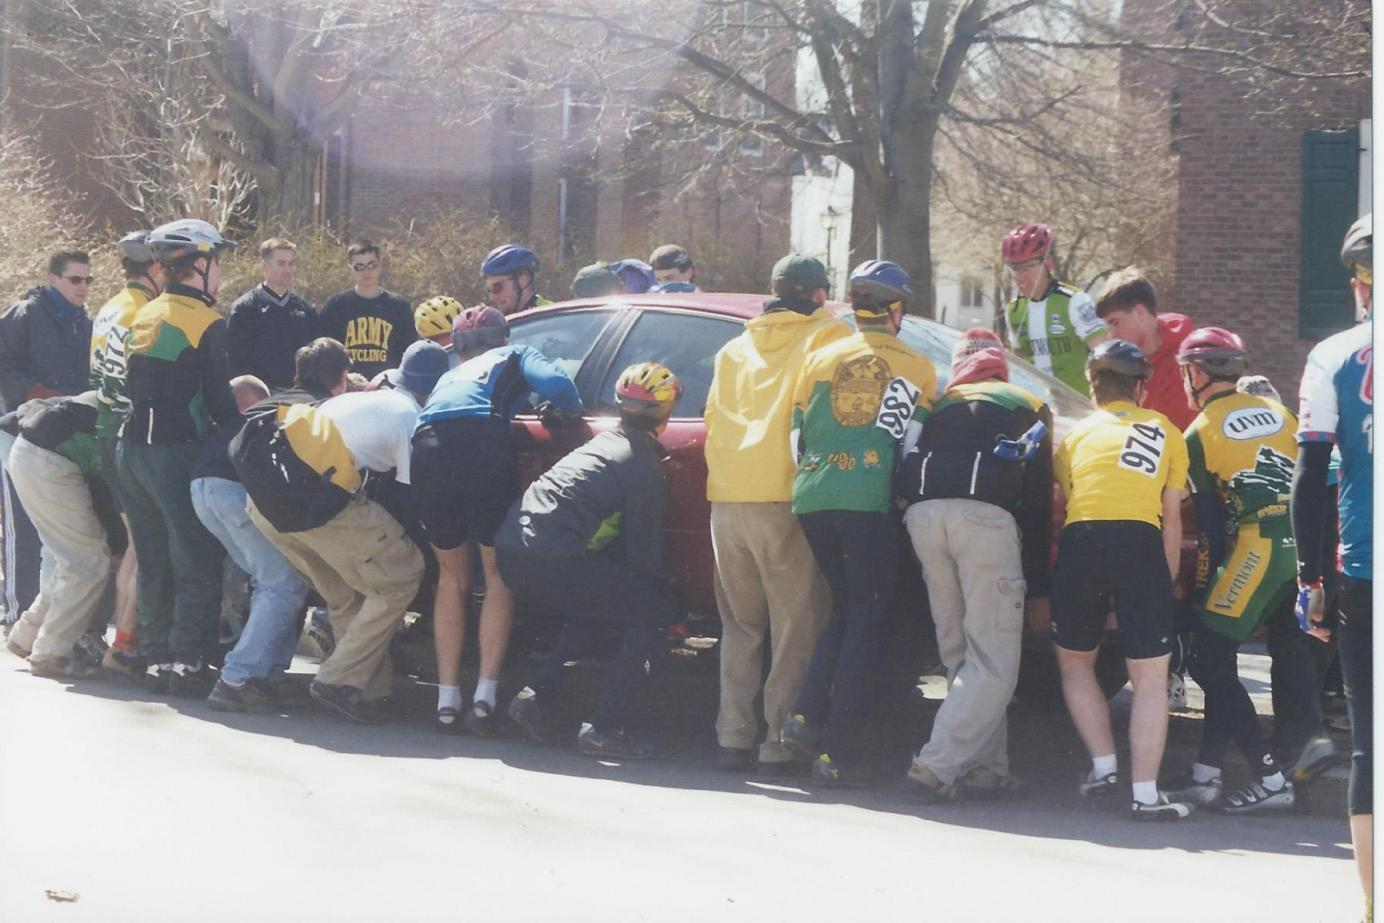
\includegraphics{dartmouth_car.jpg}
  \caption[Students moving a car off a criterium course]{
            Students moving a car off of the Darmouth criterium course
            when towing services were unavailable.\\
            Credit: Alan Atwood}
  \labfig{dartmouth_car}
\end{marginfigure}

The \pbproleref{role:primary_promoter} should call the towing company the night before the race to ensure they are still planning to clear the course -
otherwise you may have to resort to drastic measures (\reffig{dartmouth_car}) to clear the course in the morning!

\subsection{Friday Evening}

The \pbproleref{role:lead_org} and \pbproleref{role:primary_promoter} should ensure that race officials and staff are able to check in to their hotel rooms%
\sidenote{%
  You can pre-pay rooms at some hotels, so staff can just check-in by name and get a key.
  At other hotels, you may need to have an organizer check in with a credit card, and leave the keys for each person.}%
.

All traveling staff and cycling teams will trickle into the area throughout the night.
Given the large geographical size of the ECCC, people may be arriving quite late.

\subsection{Saturday Morning Setup}

The \pbproleref{role:primary_promoter} should plan to be the first person at the race, arriving at least two hours before the first race of the day
(\reffig{early_am_setup}).

\begin{marginfigure}
  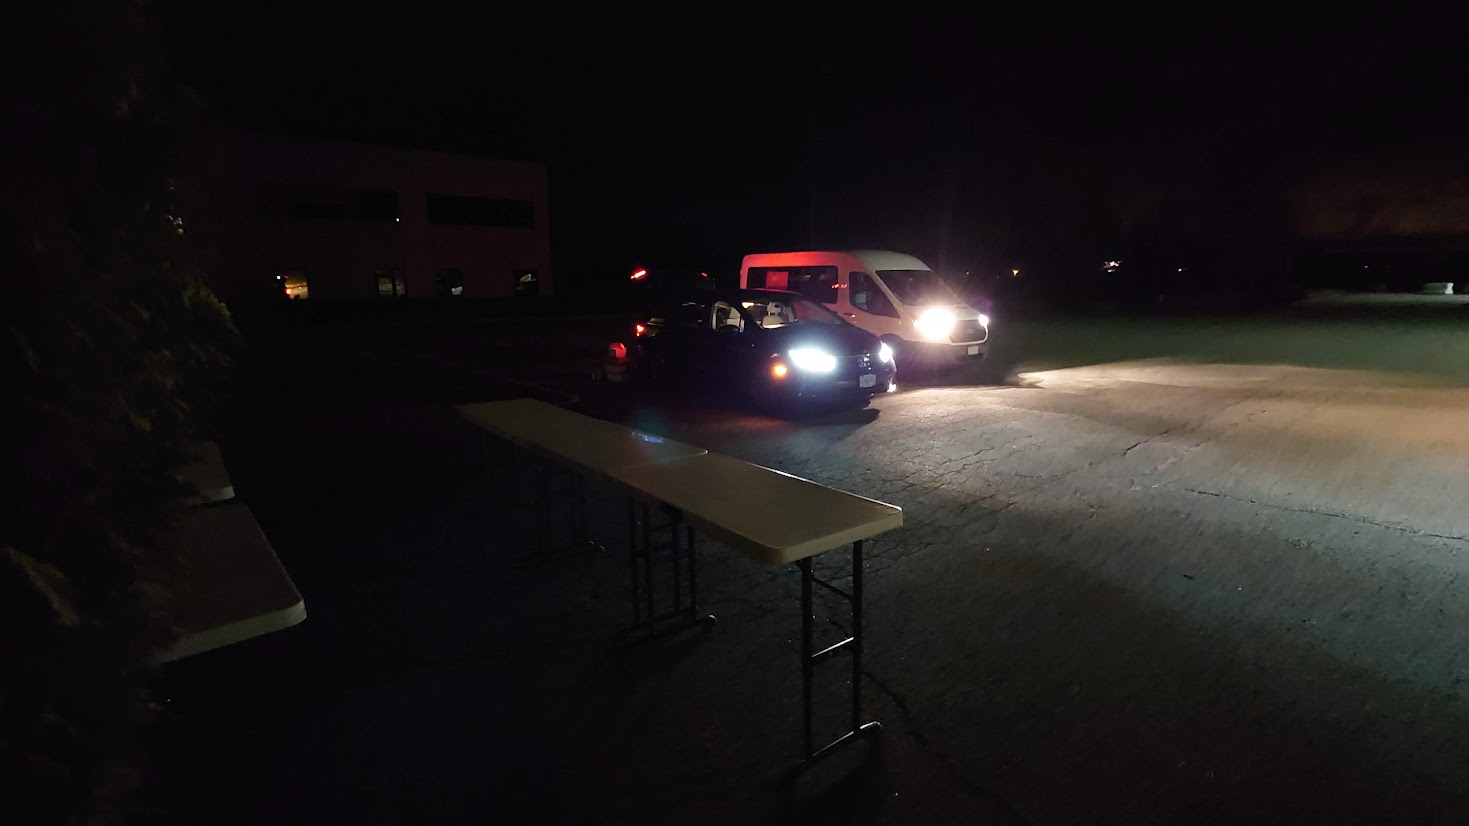
\includegraphics{2022_umass_early_am.jpg}
  \caption[Early morning race setup]{Expect to be setting up well before sunrise.\\
            Credit: Flyyn Leonard}
  \labfig{early_am_setup}
\end{marginfigure}

The \pbproleref{role:primary_promoter} should use this time to do a final check of the course,
ensuring that there are no hazards (sand on course, etc),
and that all directional signs and barriers are ready for the race.

If a location for the finish line has not been finalized, the \pbproleref{role:primary_promoter} should finalize that location now,
so the timing company, race officials, and riders can be informed of its location.

The \pbproleref{role:registrar} and \pbproleref{role:secondary_promoter} should be the next to arrive, at least 90 minutes before the first race of the day.

\subsubsection{Registration Setup}

The \pbproleref{role:registrar} should start setting up registration with assistance from the \pbproleref{role:primary_promoter} or \pbproleref{role:secondary_promoter}.

Registration must open 1 hour before the first race of the day, so setup is typically a high priority to ensure everything is ready before participants arrive.

\begin{itemize}
  \item Setup cover for registration - either hold registration inside or under the branded ECCC pop-up tent
  \item Ensure registration is locatable. If registration is under the branded ECCC tent that is typically sufficient, but if buildings block the view,
    ensure signs guide participants to registration
  \item Setup tables - typically a line of tables that participants approach, and additional tables at the back of the registration space
  \item Setup power
  \item Setup computers, printers, printers, the cash box
  \item Prepare supplies so they are easy to access: bib numbers, blank waivers, somewhere to store completed paperwork
\end{itemize}

\subsubsection{Volunteer Arrival}

The volunteer coordinator should ask that the first set of volunteers arrive between 60-90 minutes before the first race starts -
not so early that the volunteers disrupt the registration setup and first course sweep, but not too late that they need to be given directions
within the hectic hour before the first race.

\subsubsection{T-60 Minutes}

While the earlier hours are typically dark and quiet, everything starts to get busy one hour before the first race of the day starts.

Participants will start arriving in large numbers, needing help parking and directions to registration.
The \pbproleref{role:registrar} and any registration assistants will have their hands full processing registrations and handing out bib numbers,
and also being the point person that everyone asks for the day's schedule, which side to pin numbers on, and for directions to the bathrooms.

The timing company should arrive at least one hour before the first race.
The \pbproleref{role:primary_promoter} should greet them when they arrive,
and show them where the finish line is so the timing company can setup their equipment.

Race officials should be told to arrive one hour before the first race starts%
\sidenote{This is a USA Cycling standard.}.
The \pbproleref{role:primary_promoter} should meet the USA Cycling officials when they arrive.
The officials should be shown where everything is located, and the promoters should attend a briefing with the officials,
and ensure everyone is on the same page regarding communication (especially ensuring that race staff are not using a radio channel that the officials think is officials-only).

\subsubsection{T-30 Minutes}

Medical standby/EMTs should arrive around 30 minutes before the first race.
The \pbproleref{role:secondary_promoter} should meet them when they arrive,
providing them with communication methods (radios, cell phone numbers), maps, and brief them on what the day will entail.

Police detail officers should also be arriving around 30 minutes before the first race.
The \pbproleref{role:secondary_promoter} should meet and brief the officers, and ensure the officers block roads with barriers
before the race begins.

If the criterium is using a lead car, the \pbproleref{role:assistant_promoter} and Volunteer Coordinator should ensure the vehicle and driver are ready.
The \pbproleref{role:secondary_promoter} should tape a "Lead Car" sign to the front and rear windows,
give the driver a radio and a short briefing.

\subsubsection{T-20 Minutes}
\labsubsec{road_pbp_crit_t-20}

Before getting the first race lined up, the \pbproleref{role:primary_promoter} should check that everything is ready:

\begin{itemize}
  \item Are all roads closed, with proper police details and marshals ensuring a safe race?
  \item Are all hazards clear, including:
  \begin{itemize}
    \item No cars on course in dangerous locations
    \item Any dangerous potholes or sewer grates are covered
    \item Potential crash points, including telephone poles, cars, and fences are covered with hay bales or another crash barrier
  \end{itemize}
  \item Is the finish line setup and are the Timing Company and \pbproleref{role:chief_judge} ready?
  \item Is the \pbproleref{role:chief_ref} ready to start the race?
  \item Is Medical Standby ready and on-duty, and properly briefed?
  \item Did the majority of students have some issue getting to the race and registering?
\end{itemize}

If any of the above items are not ready, the \pbproleref{role:primary_promoter} should determine if races should be delayed.
If a delay is appropriate, it should be announced to all riders.

The \pbproleref{role:secondary_promoter} should work with the Volunteer Coordinator to deploy any marshals who have not already gone out,
ensuring all marshals have a safety vest, radio, and have been briefed.

\subsection[First Criterium Field]{The First Criterium Field}

\subsubsection{T-15 Minutes}

Assuming no delays%
\sidenote{See \textbf{\nameref{subsec:road_pbp_crit_t-20}}}
the \pbproleref{role:primary_promoter} should get the race ready to start:

\begin{enumerate}
  \item Communicate with the \pbproleref{role:registrar} to close registration%
    % TODO: document when to close registration as a regulation, link
    \sidenote{Registration at ECCC events traditionally closes 15 minutes before the start of the race.}
  \item Announce a first call to staging%
    \sidenote{Try to keep announcements gender-neutral: ``First call for staging for those racing in the Men's C/D field''}
\end{enumerate}

\subsubsection{T-10 Minutes}

The \pbproleref{role:chief_ref} and \pbproleref{role:secondary_promoter} should start getting riders lined up.
Each should be looking to see if any numbers are incorrectly pinned - with ten minutes, issues can be quickly addressed
without delaying the race.

The Announcer should announce a final call to staging.

\subsubsection{T-5 Minutes}

Once the majority of participants have lined up, the \pbproleref{role:primary_promoter} should record the bib numbers
of each rider on the start line.
The \pbproleref{role:primary_promoter} can record the numbers via a voice recording, typing them in to a spreadsheet,
or by using a custom app%
\sidenote{Flyyn/The Results Van are working on an app for this.}.

If any riders need to be talked to%
\sidenote{There are various reasons why riders may need to be found before starting: missing waivers or payment, unaddressed rule violations in prior races, etc.}
the \pbproleref{role:primary_promoter} should be looking for those numbers as they check the riders.

The \pbproleref{role:chief_ref} typically gives a series of announcements and rule reminders.
The \pbproleref{role:primary_promoter} should supplement the announcements with any specifics about the course or collegiate cycling points and procedures.



% \section{Brainstorming}

% Before you can start any paperwork or other preparations,
% you need to have a general idea of where you want to race.

% % TODO: move to MTB play-by-play
% %This is very easy for most mountain bike races -
% %you must have a suitable mountain (with elevation) for downhill races,
% %and Enduro and Dual Slalom races require suitable elevation and specific trails to be successful.

% \subsection{Location}

% The rough location of a race (at the scale of county, or rough area of a state)
% is often an important decision.

% Consider the following:

% \begin{enumerate}
%   \item Distance for collegiate students
%   \item Non-collegiate race audience
%   \item Local teams that could host or otherwise contribute to the race
%   \item If lodging is available nearby
% \end{enumerate}

% \subsection{Course Design}
% \index{course design}

% \subsection{Towing}
% \index{towing}

% Especially for criteriums, % TODO: ref
% cars on course can be extremely dangerous for participants.

% Even if No-Parking signs % ref
% are put up on course, local residents are still highly likely to park on course,
% and towing should always be expected.

% \begin{marginfigure}
% 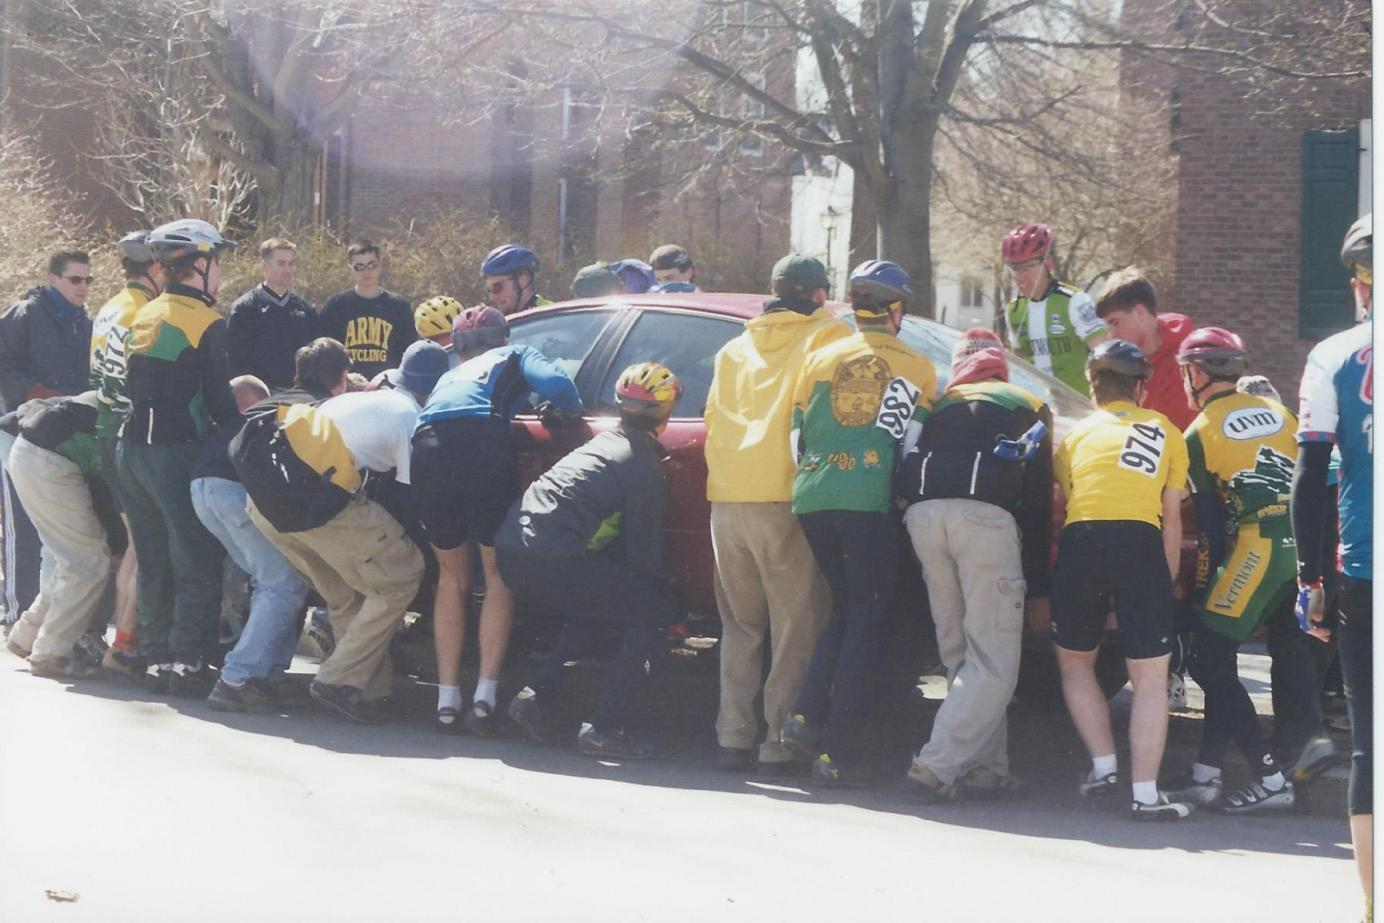
\includegraphics{dartmouth_car.jpg}
% \caption[Students moving a car off a criterium course]{
%           Students moving a car off of the Darmouth criterium course
%           when towing services were unavailable.\\
%           Credit: Alan Atwood}
% \labfig{dartmouth_car}
% \end{marginfigure}

% % TODO: legal info?

\section{Race Weekend}

The night before the race will be upon you sooner than you expect;
hopefully all of the preparations above will have been completed!

This section will walk through all the work that needs to be done for each of the days of racing.

For this example a hypothetical schedule is described with a criterium on Saturday and both a time-trial and road race scheduled for Sunday.
Weekends may look different from this example.

Additionally, a few example medical emergencies are described
(based on actual emergencies that have happened during ECCC events).

Keep in mind that emergencies may happen at any point in time -
a rider pre-riding before a race may crash and tie up all medical services before an event even has started!

% TODO: document getting hotels for race staff

\subsection{Saturday Morning Setup}

In the very early morning (\reffig{early_am_setup})
the final setup will begin.

\index{registration table}
Place tables and chairs for registration,
% TODO: a better description of ideal registration location should be written elsewhere, and referenced
ideally under an ECCC branded tent (shown in \reffig{eccc_tent}). % TODO: replace with an image of a registration setup
Depending on the setup, you may also need power,
computers, boxes for paperwork, blank forms, a printer, and more.

\begin{marginfigure}[60pt]
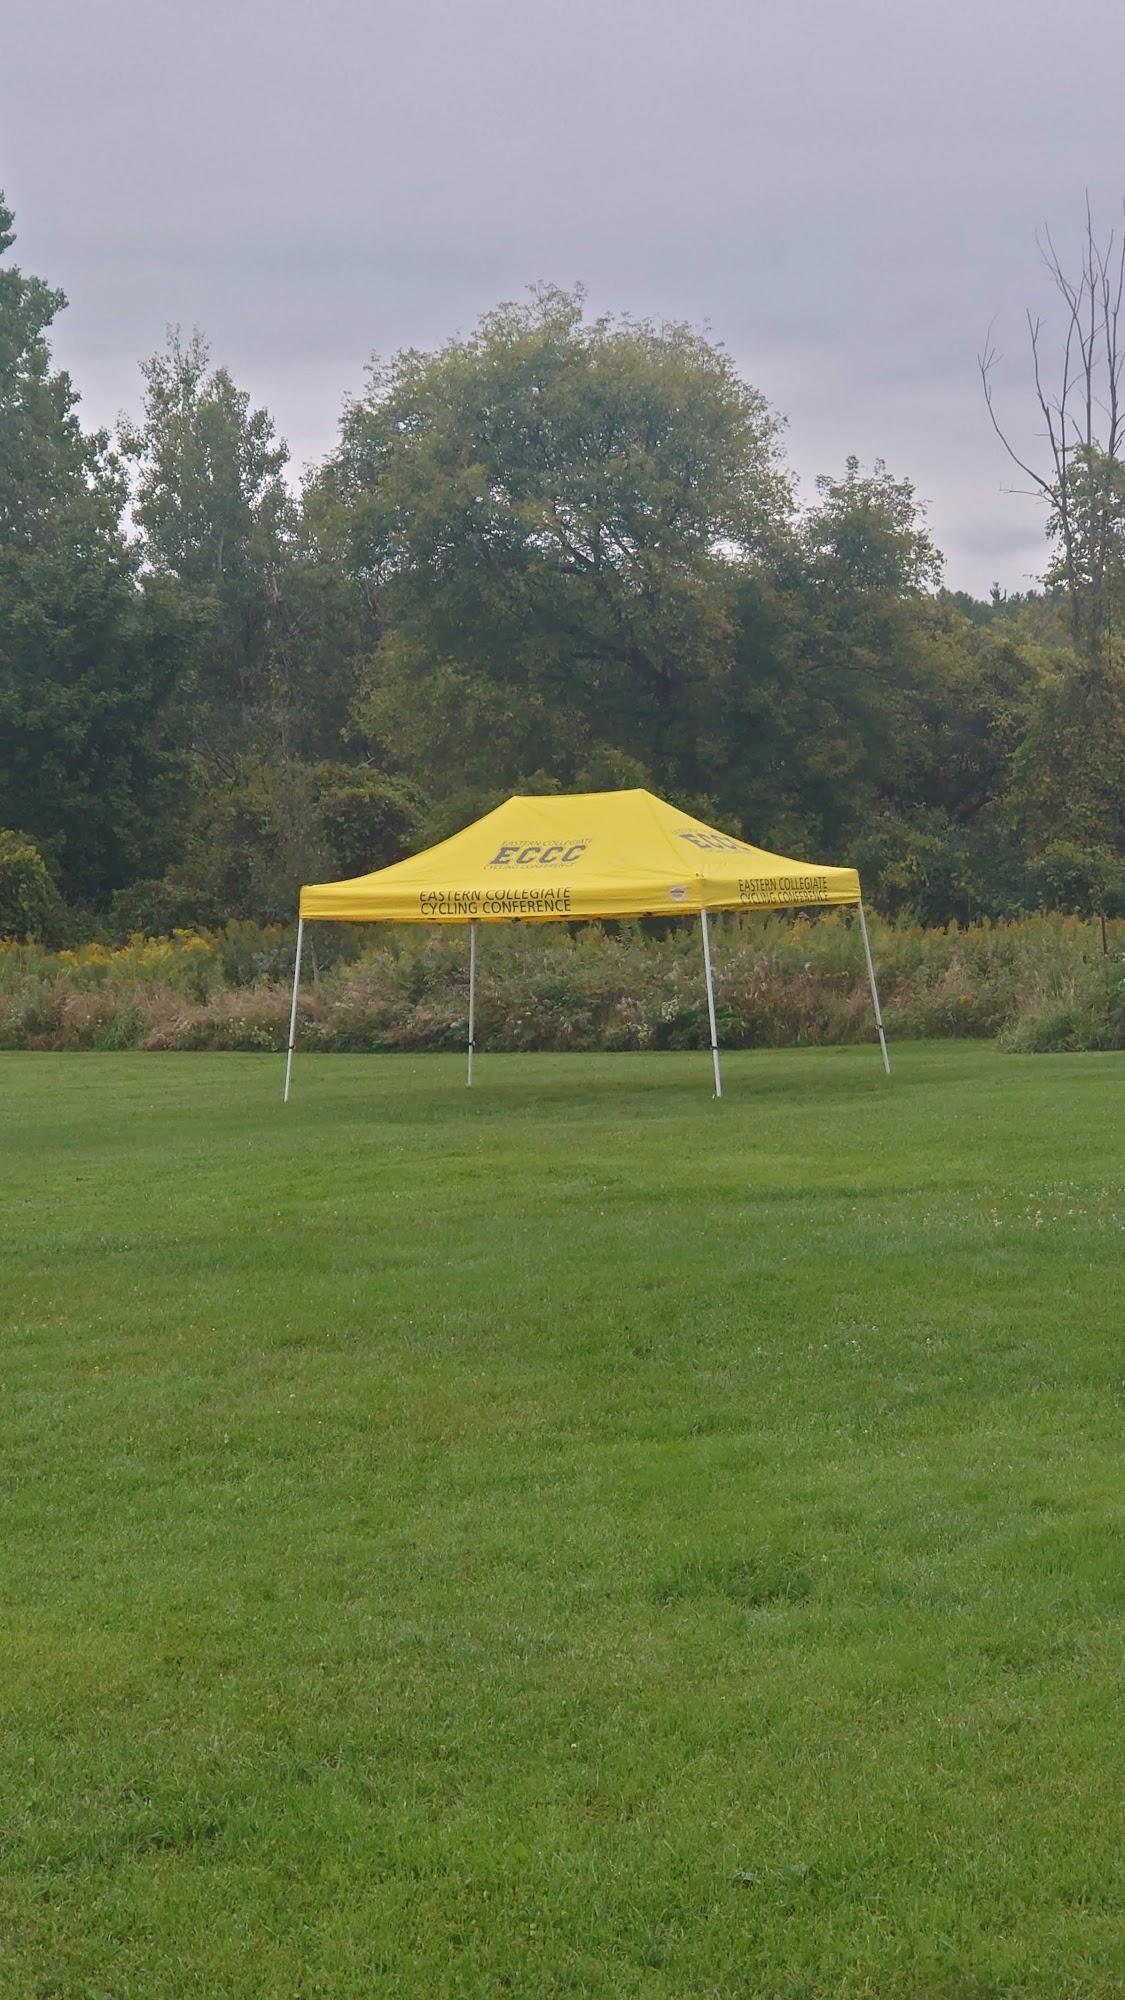
\includegraphics{eccc_tent.jpg}
\caption[The ECCC Tent]{The ECCC Tent\\
          Credit: Flyyn Leonard}
\labfig{eccc_tent}
\end{marginfigure}

If the location of the finish line has not been finalized, pick the location now.
Plan to setup a pop-up tent, table, and chairs at the finish line, unless the officials or timing company are providing their own.

Do a final course inspection:
\begin{itemize}
  \item ensure towing services have removed any cars parked on course
  \item check that navigation signs are in place
  \item check that barriers and signage for locals are in place
  \item look for any course hazards - storm drains, potholes, etc. Cover or mark with spray paint.
  % TODO: document ways to mitigate hazards, reference
\end{itemize}

\index{parking}
Ensure parking is easy to find (put up signs if necessary).
Reserve some parking for event staff.

Mark the finish with a flag, and consider putting down a line - consult with your timing company to ensure your marking does not interfere with the finish line camera.
% TODO: add figure of finish line marking

As staff and volunteers arrive, greet them and fill them in on the essentials, including where restrooms are,
and where registration, the finish line, and staging are going to be.

\index{radios}
If you are using event radios, % TODO: document somewhere, reference
distribute radios early so people already have them before they are needed.
Consider signing out equipment (like radios and safety vests) to reduce the risk of loosing items.

\subsection{Event 1: Criterium}

Most teams will have departed campus sometime Friday afternoon and slept in a hotel or with a local teammate.

About an hour or two before the first race starts,
teams will start parking and making their way to registration.

\subsubsection{Registration}

The majority of riders who come to registration fall into one of the following categories:

\begin{itemize}
  \item Pre-registered riders without a number already,
        who need to check in, turn in any paperwork, and get a number
  \item Riders who have not pre-registered,
        who need to complete waivers and other paperwork,
        pay for their race entry,
        and be assigned a number
  \item Riders who have already been assigned a number,
        but wish to register for additional races
\end{itemize}

% TODO: move the following to a formal registration section, and reference?

However, riders will also use the registration table as their primary location
for any issue, so registration should also be prepared for:

\begin{itemize}
  \item Directing riders to restrooms, staging, feed zones, the finish line, and where results will be posted
  \item Answering questions about which side numbers should be pinned on
  \item Directing any questions about rules to the officials or other staff
  \item Directing riders with minor injuries towards medical, and activating a medical response for any more major incidents that are reported to registration
  \item Directing marshals and other volunteers to the volunteer coordinator, or directly handing out safety vests, flags, and radios
\end{itemize}

\subsubsection{Road Closure}

Typically criterium courses are closed at least 30 minutes before the race starts - this prevents people from parking on course, and provides riders a safe opportunity to pre-ride the course.

\begin{kaobox}[title=Official Pre-Riding and Legal Liabilities]
% TODO: have someone (legal?) review this
\textit{This is not legal advice. Please review laws, insurance documents, USA Cycling regulations, and consult with a lawyer if you have questions.}

If you inform riders that they can pre-ride, either in the permit or verbally, your moral (and potentially legal) responsibilities have started.

Keep safety in mind.

If an injury occurs during an official pre-riding time,
ensure it is fully documented. % TODO: document incident documentation elsewhere, link
\end{kaobox}

\subsubsection{Pre-Riding}
\index{pre-riding}

\subsubsection{Setup}

\begin{enumerate}
  \item Pit
  \item Finish line timing provider
  \item Finish line officials
  \item Lead car/motorcycle (if used)
  \item Medical
\end{enumerate}

\subsubsection{Start Line}

% TODO: mention setting up PA system earlier in document

Roughly 30 minutes % TODO: 30?
before the start of the first race, there should be an announced ``first call to staging''.

\begin{marginfigure}
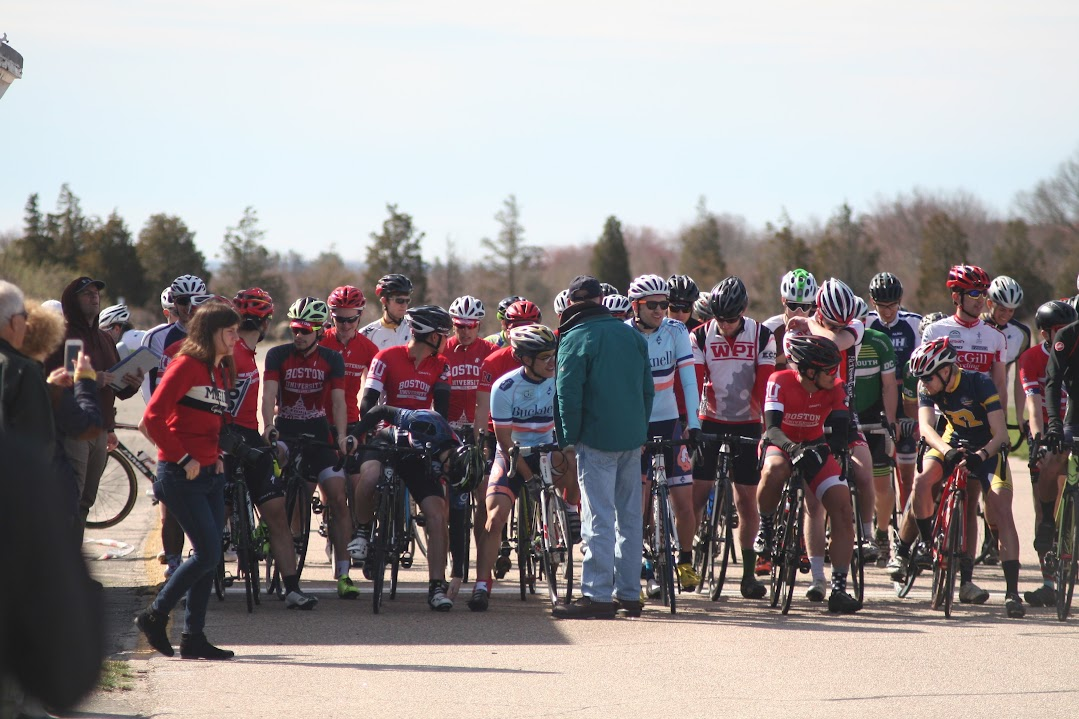
\includegraphics{2017_start_line.jpg}
\caption[Riders lined up at a criterium start line]{
          Riders lined up at the start line for the 2017 Ninigret criterium.\\
          Credit: Flyyn Leonard}
\labfig{criterium_start_line}
\end{marginfigure}

At this point, any lead car or follow official motorcycle should be prepared.
The officials and a race representative should make their way to the staging area/start line.

The chief referee will ensure that they have an official in the pit, and the race organizers should check that marshals are deployed to all corners, course crossings, and any other notable spots.

\subsubsection{Racing}

The whistle blows, and the riders charge off the start line.

% TODO: if start line is a common incident spot, mention

\subsubsection{Beginner's Clinic}

All ECCC criteriums should feature a
beginner's clinic% TODO: document in regulations, link
\sidenote{
Not only do beginners clinics provide the experience we want for new riders,
USA Cycling discounts permitting fees for races that include a beginner's clinic.
}%
.

% TODO: include picture of a clinic

45-60 minutes before the clinic is scheduled to start,
have clinic staff meet and hold a short briefing meeting.
Ensure all clinic staff receive a safety vest.

Inspect the location where the clinic will meet - if one was not picked in advance, quickly find a location at this point.
Ensure the registration table also knows where the clinic will be, as riders frequently ask.

15-30 minutes before the clinic is scheduled to start,
announce the clinic, ensuring to mention where participants should meet.

The clinic should have at least 30-60 minutes of off-course instruction and drills.

Following the drills, the clinic should have a scheduled period when no riders are on course, and the clinic should practice riding around on the course,
and practice cornering on the actual course corners.

This clinic on-course practice time is a good period for the USA Cycling officials and timing company to get a break!

\subsubsection{Beginner Races}

Following the clinic's off-course and on-course sections,
beginner races should be scheduled.

% TODO: include picture of clinic staff

Clinic staff should ride at the back of the beginner race,
providing coaching and support to any riders who need it.

% TODO: Describe the beginner race

\subsubsection{Emergency: Crash}

\subsection{Sunday Morning Setup}

\subsection{Event 2: Time Trial}

\subsection{Event 3: Road Race}

\subsubsection{Marshal Deployment}

\subsubsection{Caravan Preparation}

\subsubsection{Start Line}

\subsubsection{On-Course}

\subsubsection{Emergency: Crash}

\subsubsection{First Rider In}

\subsubsection{Sweep}

\subsection{Course Cleanup}

\section{Post-Event Financial}

\section{Post-Event Paperwork}

\setchapterstyle{kao}
\setchapterpreamble[u]{\margintoc}
\chapter{MTB Race Play-By-Play}
\labch{mtb-play-by-play}

% TODO: create section similar to Road Race Play-by-Play
% First section: brainstorming

\pagelayout{wide}
\addpart{Regulations}
\pagelayout{margin}

\setchapterpreamble[u]{\margintoc}
\chapter{Race Hosting}
\labch{hosting}

\section{Team-Hosted Events}
\labsec{hosting:team}

There is a long-held expectation in cycling that teams who attend races host events themselves,
contributing to the local racing community.

Teams who successfully organize races:
\begin{enumerate}
  \item provide an opportunity for people to race - if it wasn't for other teams hosting events, you wouldn't get to race yourself
  \item enhance their reputation as a team
  \item have an opportunity to promote their sponsors at the event
  \item have stronger teams by uniting their members in a common project
  \item earn money, via whatever profit is made from the event
\end{enumerate}

Historically, hosting races has been an expectation of collegiate teams as well.

However, recent years have seen a sharp decline in the commitment from teams to run events,
so conferences (including the Eastern Collegiate Cycling Conference) have struggled to run seasons.

For some seasons, the ECCC has started to host their own events, % TODO: hyperlink
and other conferences (such as the SECCC) have had to turn to outside companies to run their seasons, % TODO: hyperlink
increasing costs and sacrificing some of the collegiate atmosphere.

\subsection{Finances and Budget}
\labsubsec{hosting:team:finance}

In a team-hosted race, the organizing collegiate team is responsible for the budget and finances for the race (although the ECCC is here to advise, and has some emergency funds in some circumstances).

The hosting team will be paying for the expenses to run the event:
\begin{itemize}
  \item Venue fees, if applicable
  \item Signage, caution tape, and other course equipment as needed
  \item Permitting fees
  \item Services used at the race, including:
  \begin{itemize}
      \item Officiating
      \item Timing services
      \item Registration services
      \item Medical providers, such as EMTs and bike patrol
      \item Police details
      \item ECCC coordination fees
  \end{itemize}
  \item An ECCC surcharge
\end{itemize}

\subsubsection{ECCC Specific Costs}

There are three areas where money may need to be budgeted as going directly to the ECCC or ECCC staff members.

The exact values that the ECCC charges varies each season - contact your season coordinator and conference director for the current schedule of fees.

\begin{description}
  \item[ECCC Surcharge]
      The ECCC may specify a fixed and/or per-rider expense as an ECCC surcharge, that goes directly to the conference.

      These funds are used to pay for conference equipment that is used at races (including timing equipment, registration equipment, radios, and tents),
      and can also go towards our emergency fund used to prevent schools from loosing too much money hosting races, or to pay for races canceled due to natural disasters or pandemics.
  \item[ECCC Staff Fees]
      The season coordinator, conference director, and associated staff members may charge teams a fee for their work before and during the event.
  \item[ECCC Labor]
      In addition to the work the season coordinator and conference director do to support race organization and oversee the event,
      some events find it most effective to pay ECCC staff members to provide event services in addition to their other duties.

      For example, collegiate mountain weekends typically pay the season coordinator to work as the chief referee in addition to their work running the race day.
\end{description}

\section{Conference-Hosted Events}
\labsec{hosting:conference}

\section{External Races}
\labsec{hosting:external}

\section[Professionally Hosted]{Professionally Hosted Races or Series}
\labsec{hosting:pro}

\setchapterpreamble[u]{\margintoc}
\chapter{Race Formats}
\labch{formats}

In general, the Eastern Collegiate Cycling Conference
runs event disciplines and formats that are specified and defined by USA Cycling.

This section lists several event formats including
common formats seen in the ECCC, however there are additional
formats that could be considered.

\section{Road Events}

Each ECCC road season weekend traditionally runs three events:

\begin{itemize}
  \item A long-format race (see \nrefsubsec{format:rr})
  \item A shorter-format race, such as a criterium (see \refsubsec{format:crit})
  \item A time trial,
      commonly an individual time trial (ITT)
      or a team time trial (TTT),
      but could also be a hill climb (\refsubsec{format:hill_climb})
\end{itemize}

Either the road race or criterium could be replaced by a circuit race (\refsubsec{format:circuit}) if the roads are more suitable for that format.

\subsection{Criterium}
\labsubsec{format:crit}

\subsection{Road Race}
\labsubsec{format:rr}

\subsection{Circuit Race}
\labsubsec{format:circuit}

\subsection{Time Trial}

\subsection{Hill Climb}
\labsubsec{format:hill_climb}

Hill climbs are point-to-point individual time trials that have a significant gain in elevation.

\section{MTB Events}

Each ECCC mountain bike season traditionally contains five events:

\begin{itemize}
  \item Two cross-country races:
  \begin{itemize}
      \item One long distance Cross-Country (XC) race (\refsubsec{format:xc})
      \item One Short-Track Cross-Country (STXC) race (\refsubsec{format:stxc})
  \end{itemize}
  \item A team relay race (\refsubsec{format:relay})
  \item Two gravity races, which can be any of:
  \begin{itemize}
      \item Downhill (DH) (\refsubsec{format:dh})
      \item Dual Slalom (DS) (\refsubsec{format:ds})
      \item Enduro (\refsubsec{format:enduro})
      \item Super Downhill (Super-D) (\refsubsec{format:superd})
  \end{itemize}
\end{itemize}

\subsection{Cross-Country}
\labsubsec{format:xc}

Cross-Country mountain bike races are long-distance races,
timed and run similarly to road races. % TODO: link to road race

\subsection{Short-Track Cross-Country}
\labsubsec{format:stxc}

\begin{marginfigure}
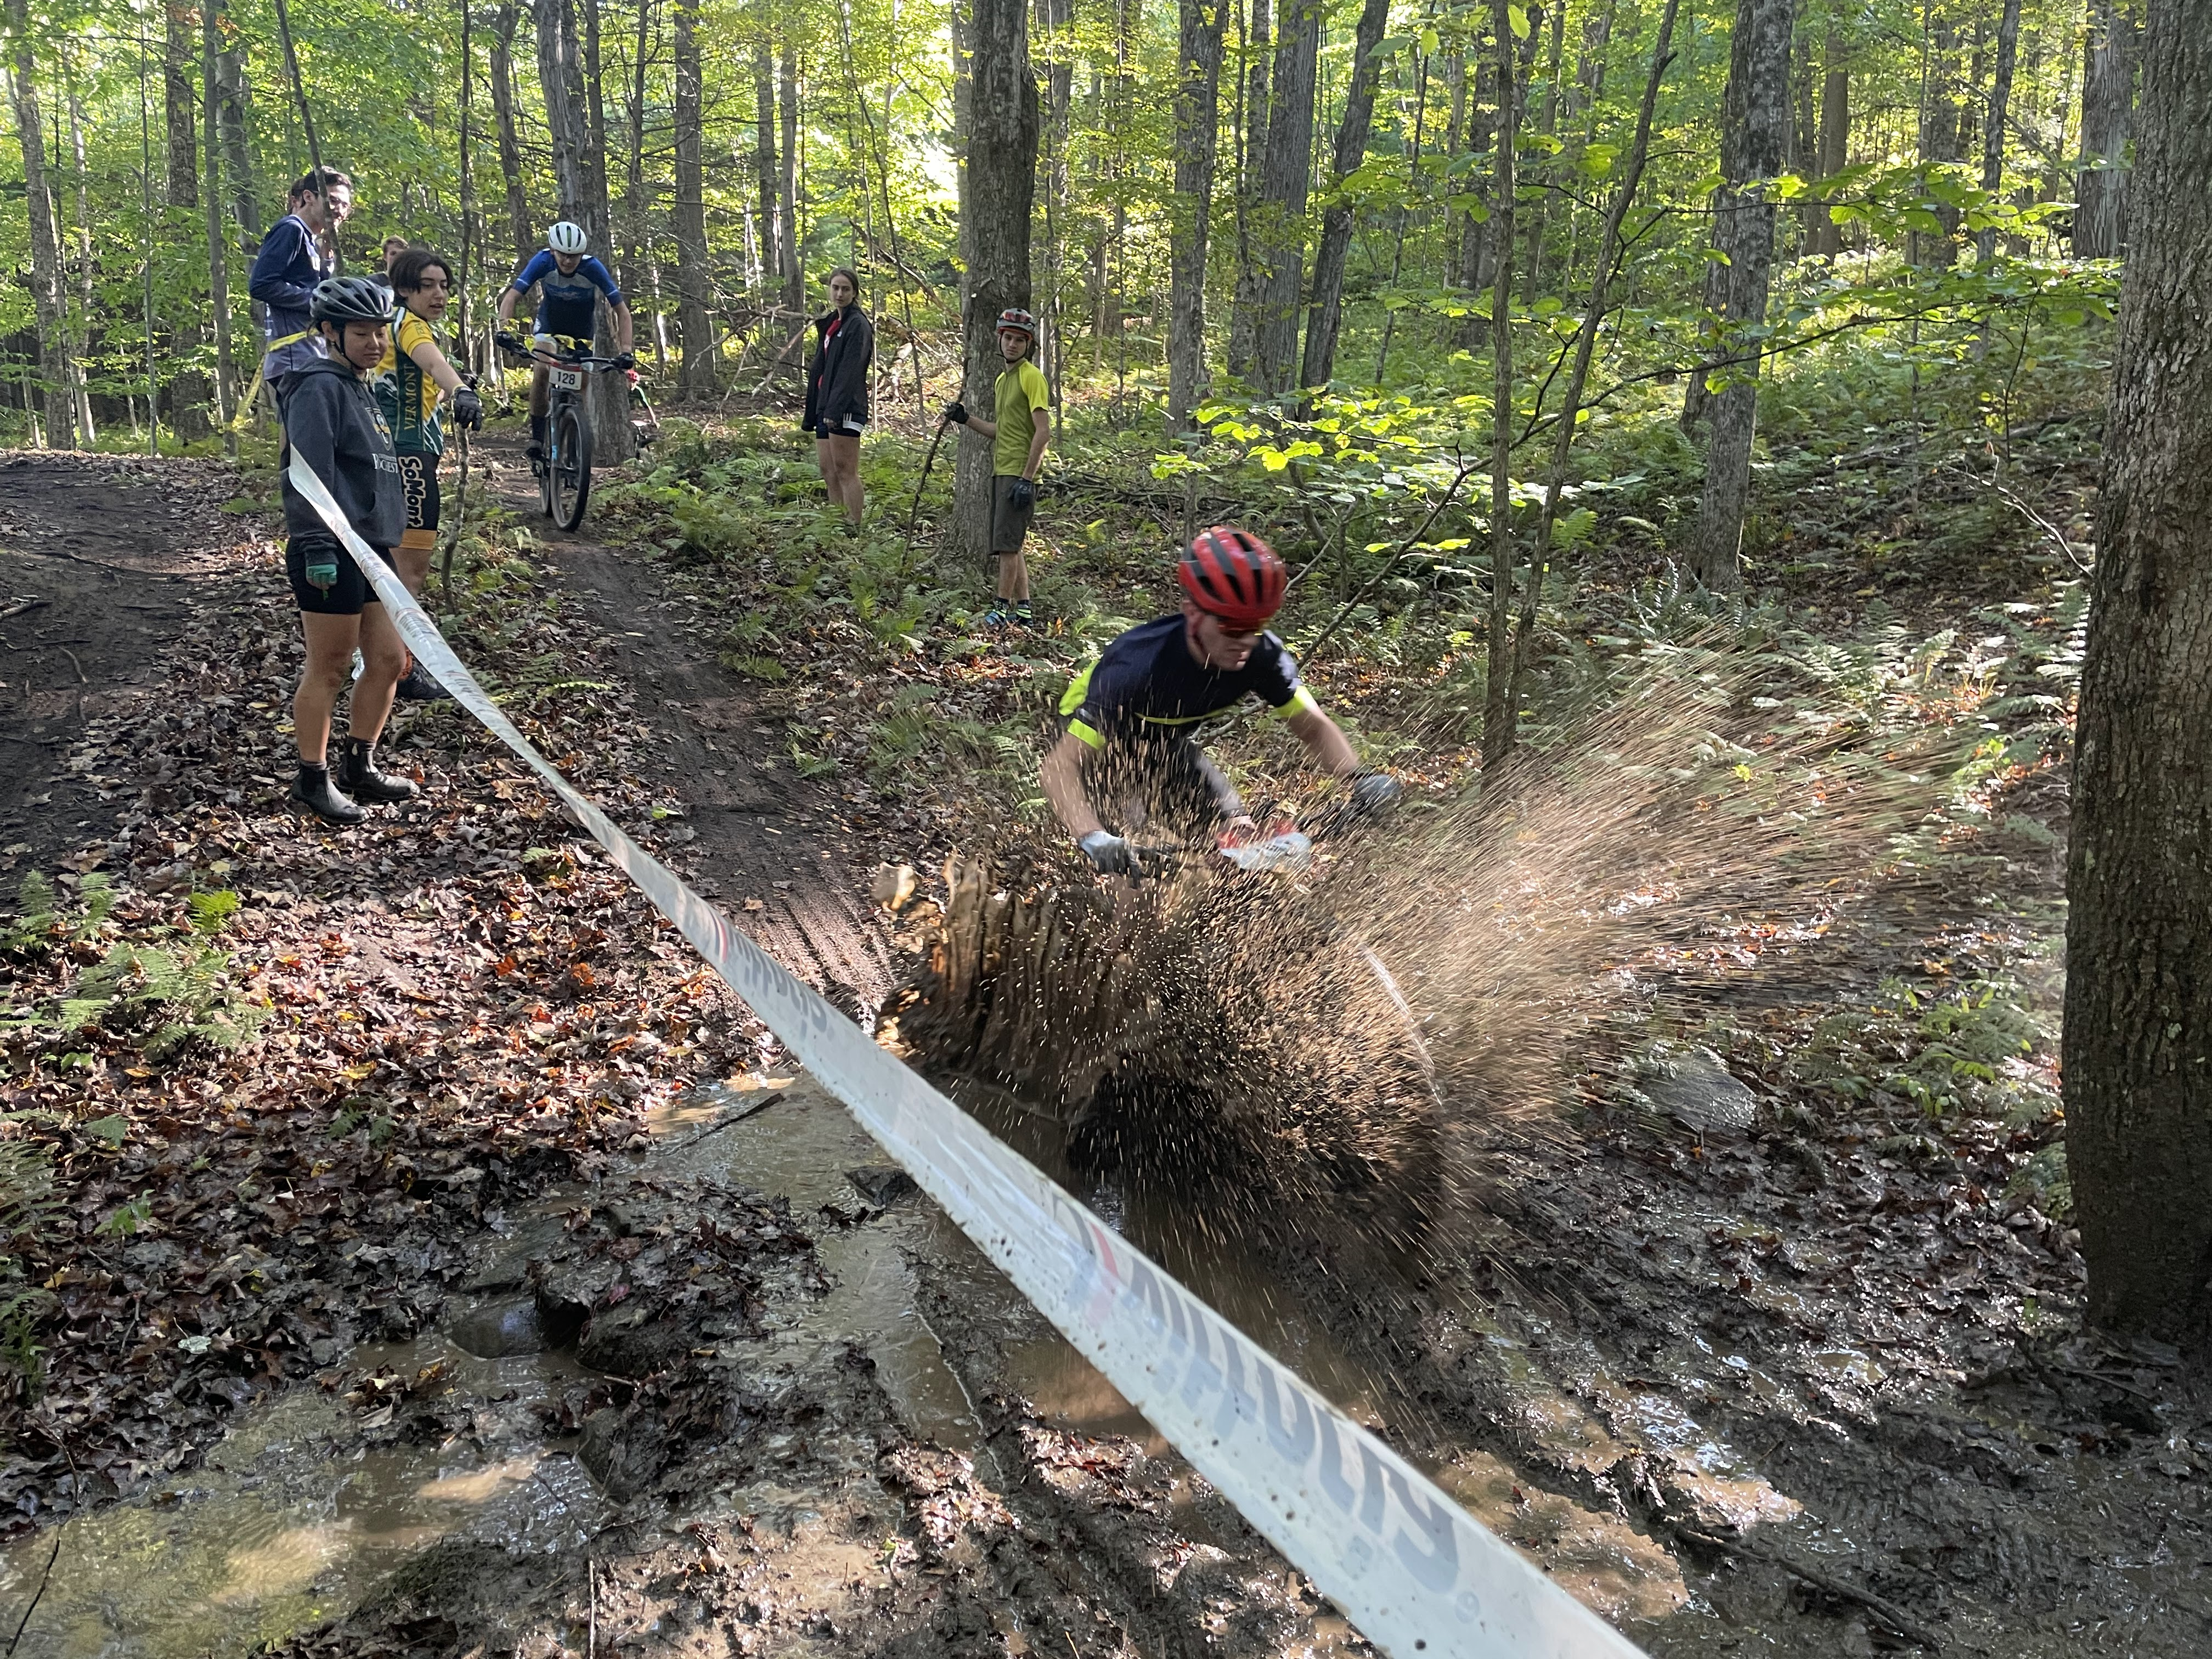
\includegraphics{IMG_9720.jpg}
\caption[A Short-Track Cross-Country Race]{A Short-Track Cross-Country Race.\\
          Credit: Cory Puckett}
\labfig{stxc}
\end{marginfigure}

Short-Track Cross-Country races are the off-road equivalent
to a criterium. % TODO: link to criterium

\subsection{Team Relay}
\labsubsec{format:relay}

Team relay races are team events, typically using the same race course as the Short-Track Cross-Country race, and are often scheduled as following the last STXC field.

\subsection{Dual Slalom}
\labsubsec{format:ds}

Dual Slalom races are short, downhill races that occur on similar, parallel courses.

\subsection{Downhill}
\labsubsec{format:dh}

\subsection{Enduro}
\labsubsec{format:enduro}

\subsection{Super-Downhill}
\labsubsec{format:superd}

\section{Cyclocross Events}

\section{Track Events}

\section{Gravel Events}

\setchapterpreamble[u]{\margintoc}
\chapter{Race Services}
\labch{services}

\section{Medical Services}
\index{EMT}

Every race should have a plan for medical emergencies
which typically includes hiring an EMT % TODO: "EMT" glossary
for event standby services, % TODO: put "event standby services" in glossary and/or markup?
having bike/ski patrol at the event,
or otherwise having someone with medical knowledge on alert.

\begin{kaobox}[title=Local EMT Knowledge]
Flyyn Leonard % TODO: macro for inserting position, e.g. \reftitle{flyyn} => Flyyn Leonard (Conference Director)?
is an EMT
and can help with questions event organizers may have
regarding medical services.
\end{kaobox}

\begin{marginfigure}
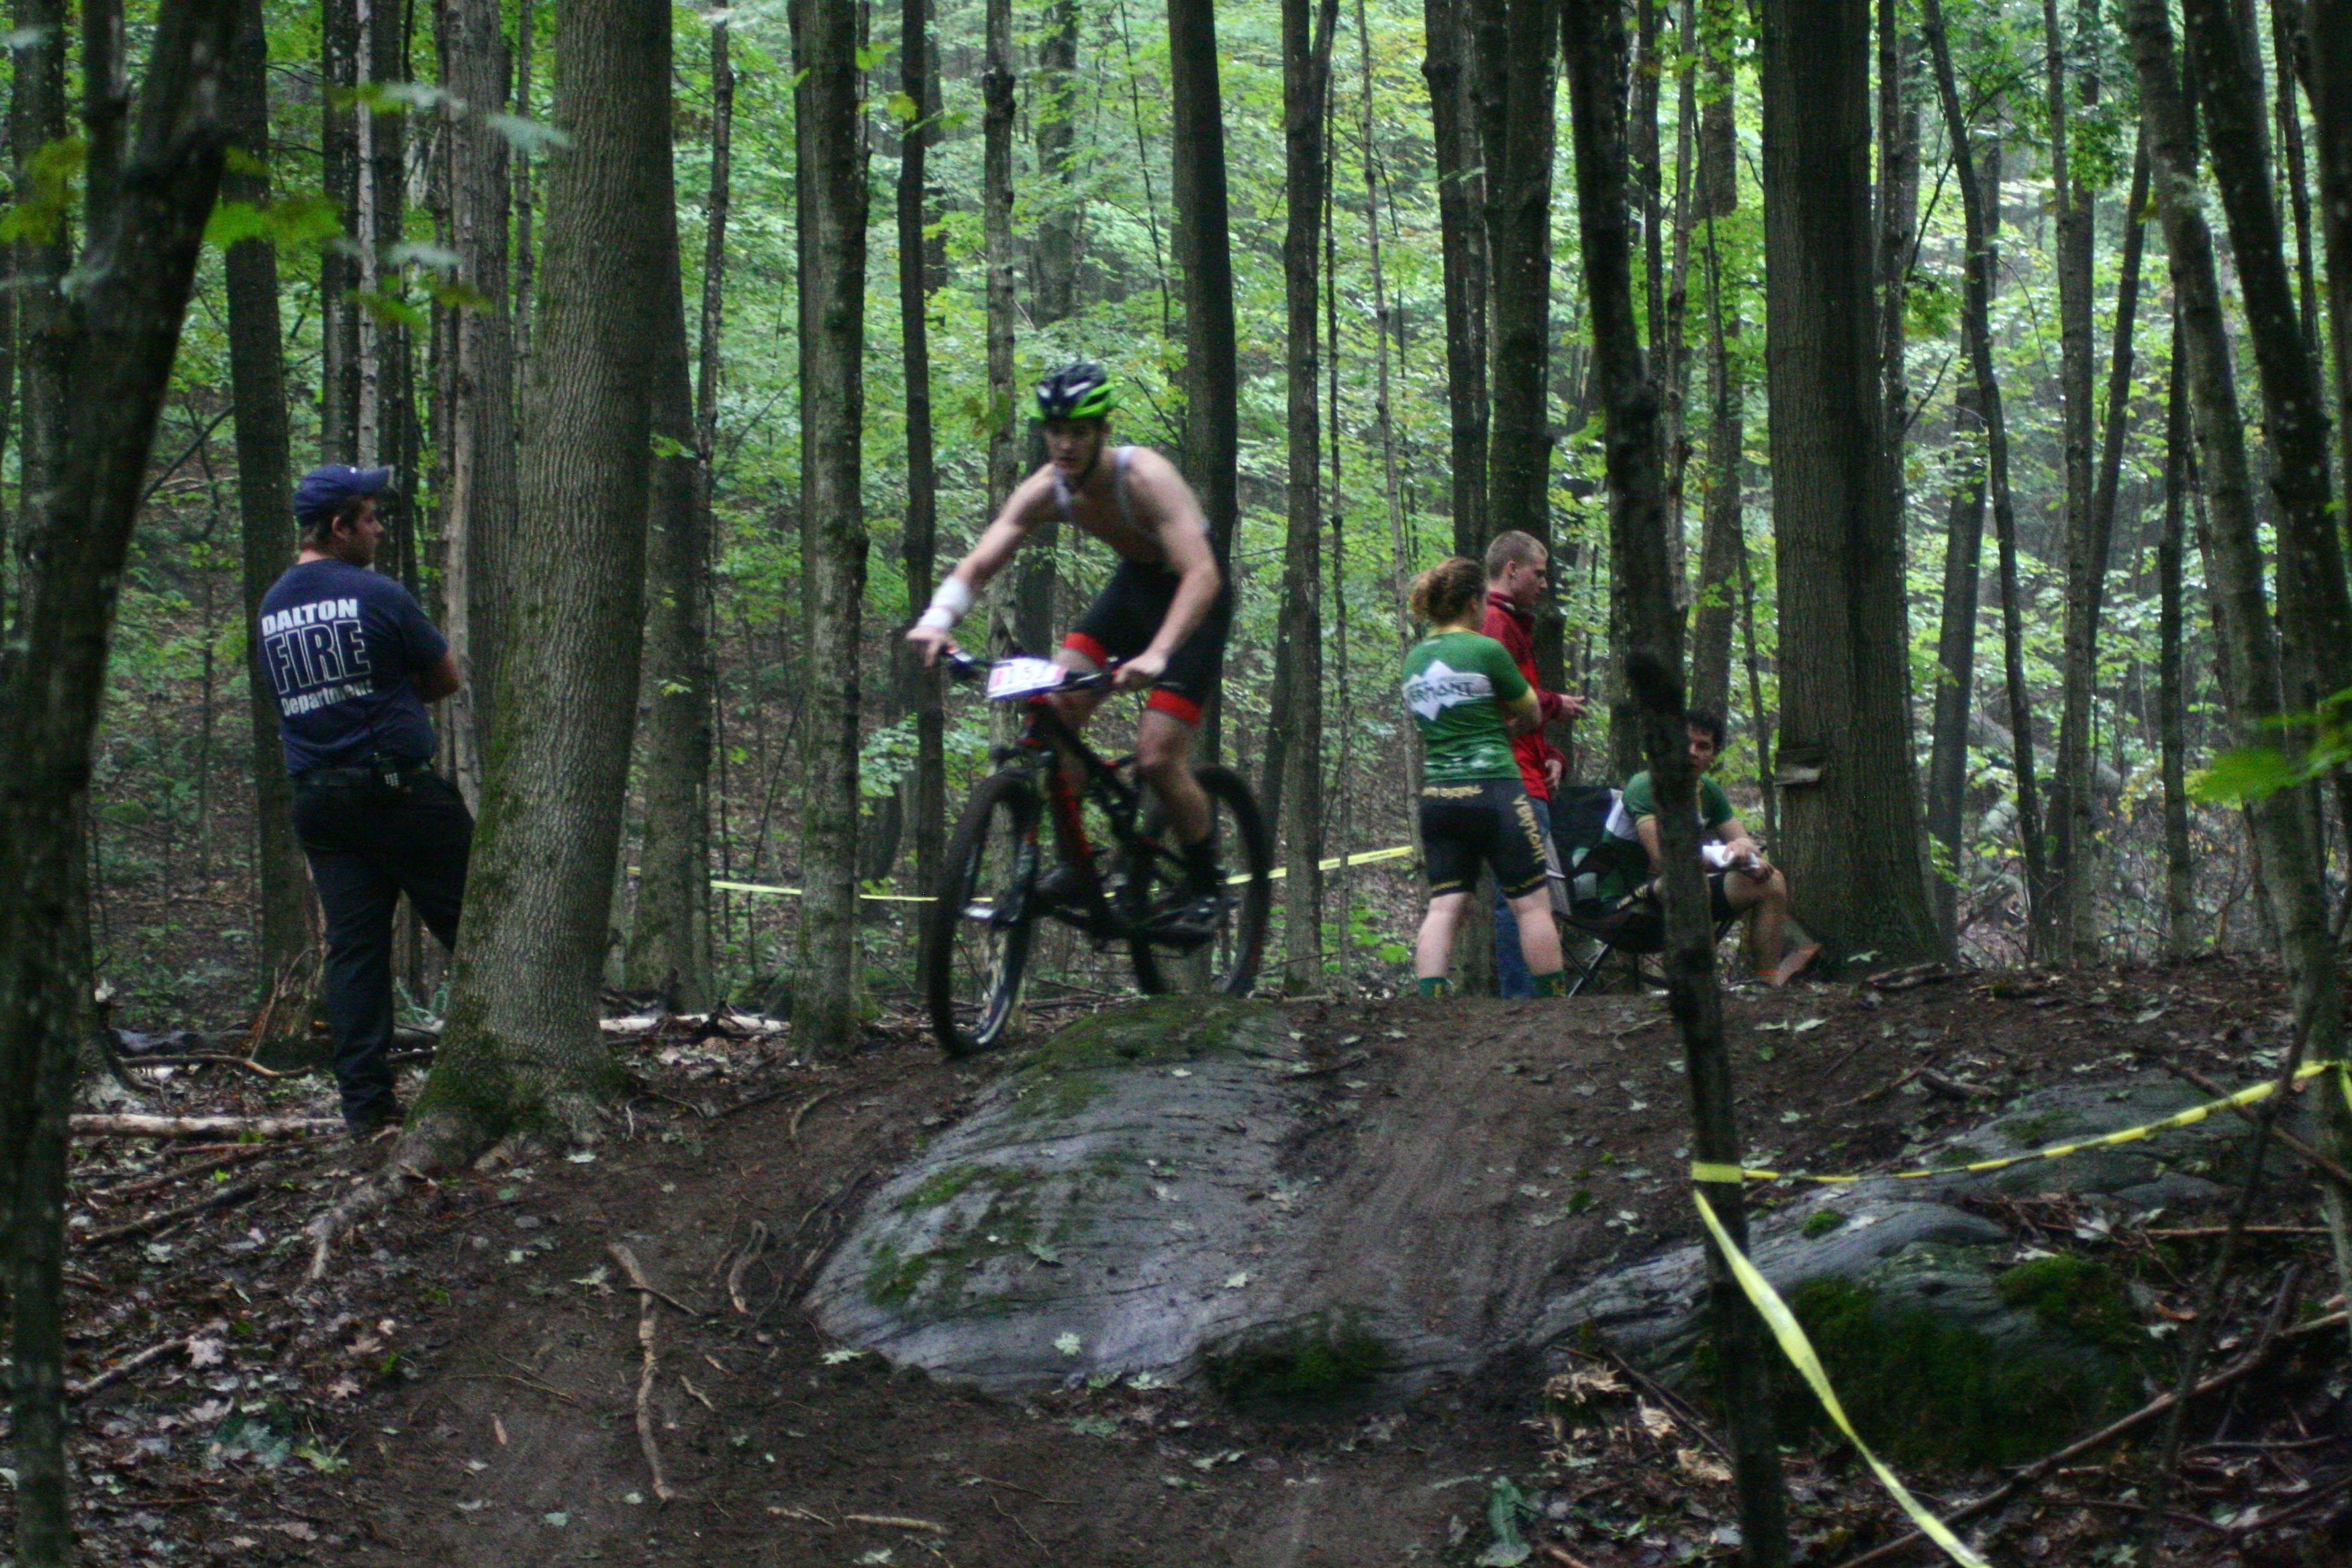
\includegraphics{IMG_5836.jpg}
\caption[Medical Standby]{A member of the Dalton Fire Department on a medical standby detail.\\
          Credit: Flyyn Leonard}
\labfig{standby}
\end{marginfigure}

% \nameref{regulation:medical}

\begin{regulation}[
  ref=medical,
  title=Required Medical Services at ECCC Races,
  draft=true
]
\begin{enumerate}[label=\Alph*.]
  \item
    All ECCC races must make every effort to obtain one or more
    properly licensed, on-duty medical providers (EMT, Advanced EMT, or Paramedic)
    who will be at the race throughout all events.
  \item
    All ECCC races must have at least one person focused on providing first-aid who has some medical or first-aid training.
    This person may be an on-duty member of a bike patrol program, an off-duty EMT, or someone who has completed a Wilderness First Responder course.
\end{enumerate}
\end{regulation}

\subsection{EMS Legal}

\subsection[Contracting]{Contracting EMS Services}

\subsection[EMS Coordination]{Coordination with EMS Providers}

You should request that your medical providers (e.g. EMTs)
arrive at the event before the first race starts -
this ensures the race can start with medical services available,
and gives the promoter time to connect and coordinate with the specific EMT
that covers the event.

You should not expect EMTs to have knowledge of the schedule, event details, or
know anything about bike racing or sports in general.

You should provide EMTs with a schedule of the day and a flyer with basic information
and an event radio (or some other way to communicate with marshals and event staff).
You may also want to provide a quick fact sheet specifically for EMTs - an example is in
\nrefch{med_guide}.

\subsection{Documentation and HIPAA}
\index{HIPAA}

\section{Officiating Services}
\index{officiating}

Officials are essential to an event.
% TODO: description of how

If your event is sanctioned % TODO: glossary
under USA Cycling
you must have a certain number of qualified USA Cycling officials working.

\subsection{Required Officials}

The number of officials varies based on the event and format.

\subsubsection{Mountain Officiating}

\begin{marginfigure}
\includegraphics[angle=270]{PXL_20211003_160518310.jpg}
\caption[MTB STXC Finish Line]{
          A Short-Track Cross Country % TODO: ref
          finish line can be run with a very small crew.\\
          Credit: Katie Aman}
\labfig{standby}
\end{marginfigure}

ECCC MTB races can typically get by with just one chief referee
(traditionally the season coordinator, e.g. Flyyn Leonard)
and a second official or timing assistant,
although additional help is always appreciated.

\begin{kaobox}[title=Note for Team-Hosted MTB Races]
You will need the following officiating resources:

\begin{itemize}
  \item Budget for a USA Cycling Chief Referee (typically Flyyn Leonard)
  \item Budget for a USA Cycling Chief Judge (or otherwise have an experienced official)
  \item Plan to have two volunteers as assistant timers for most events
\end{itemize}
\end{kaobox}

\section{Timing Services}

\section{Registration Services}

\section{Police Services}
\index{police}

\setchapterpreamble[u]{\margintoc}
\chapter{Roles}
\labch{roles}

The following roles are positions often held by collegiate students and the ECCC volunteers
when planning and running ECCC events.

Each roles is documented here with a summary of the position
and the various requirements and expectations that come with the role
so everyone knows what the role entails.

\section{ECCC Season Coordination Team}
\label{role:eccc_coordination_team}

Each collegiate cycling discipline raced in the ECCC has a set of staff members associated, led by
a \nsubsecref{role:eccc_season_coordinator}.

The \nsubsecref{role:eccc_director} oversees all season coordinators, and is available if students or staff have any questions.

% TODO: could use \begin{table} instead of \begin{figure}, but currently using figure as there are few tables,
% so there will be consistency as all included items are called "figure" and this will show up in the "List of Figures"
% Re-evaluate if there are many tables added.
\begin{figure}[h]
  \caption{Current list of volunteers holding ECCC season coordination positions}
  \labfig{season_staff}
  \begin{tabular}{c | c | c | c | c}
    \toprule
    &
    Road &
    Mountain &
    Cyclocross & Track
    \\
    %
    \midrule
    Season &
    Spring &
    Early Fall &
    Late Fall &
    Summer \\
    \midrule \\
    %
    Coordinator &
    \makecell{Benjamin Kramer \\ Flyyn Leonard \textit{(interim)}} &
    Flyyn Leonard
    & Luke Knisley
    & Flyyn Leonard \textit{(interim)} \\
    %
    Assistant Coordinator &
    Luke Knisley &
    \makecell{Luke Knisley \\ Thomas Carter} &
    Benjamin Kramer & \\
    %
    Additional Coordinators & & & &
    \bottomrule
  \end{tabular}
\end{figure}

\subsection{ECCC Conference Director}
\label{role:eccc_director}
\labsubsec{role:eccc_director}

\subsection{ECCC Season Coordinator}
\label{role:eccc_season_coordinator}

The ECCC Season Coordinator for each raced discipline is responsible for:
\begin{itemize}
  \item Guiding the direction of collegiate cycling in the respective discipline, for the ECCC region
  \item Growing and promoting cycling in the respective discipline, inside and outside of collegiate cycling
  \item Overseeing a racing season for the respective discipline
  \item Ensuring that there is an ECCC presence at each event throughout the racing season,
    to help riders with questions at the event and regarding the season,
    and ensuring a consistent and fun racing experience
  \item Assisting the ECCC Upgrades Coordinators to correctly place participants in the correct collegiate cycling racing category,
    ensuring competitive categories and safe racing
  \item Assisting the ECCC Conference Director in eligibility for national level events
\end{itemize}




\pagelayout{wide}
\addpart{Participant Guide}
\pagelayout{margin}

\pagelayout{wide}
\addpart{Team Hosting Guide}
\pagelayout{margin}

\setchapterpreamble[u]{\margintoc}
\chapter{Overview of Team Hosting}
\labch{team_host_overview}

\begin{kaobox}[title=Scope]
This section focuses on
Team-Hosted Events % TODO: properly reference, but name-first style
for road and mountain bike seasons.

Some of the items in the following chapters will only be applicable
for either road or mountain events - for example, ECCC MTB races are typically
officiated by the season coordinator with some assistants, instead of hiring an
entire USA Cycling officiating team.
Sections that are only applicable to certain types of events will be noted as such.

For conference hosted events % TODO: properly reference
please see \nrefch{conference_event:overview},
which focuses on specifically the parts of race organizing
that will be delegated to teams.
\end{kaobox}

\section{Introduction}

Thank you for your interest in hosting a race -
teams hosting races is essential for a healthy cycling community,
especially in collegiate cycling%
\sidenote{This is discussed in detail in \nrefsec{hosting:team}}.

In general, hosting a race is moderately straightforward:
you design a race, fill out paperwork, hire services.
Riders show up, you organize marshals, then registration, officials,
and the timing company run most of the racing.
After that, there's just cleanup and some concluding paperwork.

However, there are a lot of tasks to be done,
and there are a lot of hands needed on the day of the race.

Anyone can host a race - there's no special skills needed,
and our ECCC staff and this document will walk you through every step of the way.

Running a successful race can be rewarding in many ways:
\begin{itemize}
  \item You will be giving back to the cycling community,
        specifically assisting collegiate cycling
  \item Running a race can raise funds for your team
  \item Event organization is a success that you can be proud of (and list on a resume)
\end{itemize}

\section{Steps for Success}

\subsubsection{Divide the load}
Given the number of tasks that must be done, the most successful races often
utilize a large group of people to help spread the work out.

If you are on a large cycling team you may immediately have all the hands you need.
Otherwise if you are on a smaller team, you may want to reach out to teams at other colleges, or even get assistance from local non-collegiate teams.

Consider getting assistance from other sports or outdoor clubs at your school.

\subsubsection{Ask for help}

\subsubsection{Stay ahead of deadlines}

\subsubsection{Confirm everything}

Even members of our ECCC team have made assumptions about
race courses, volunteer commitments, and availability of resources provided by contracted companies.

Even if you've paid to rent a ski mountain for a downhill race,
confirm that they will have members of ski patrol handing medical standby.

\subsubsection{Have contingency plans}

Imagine it is mid-day on Friday, with only a few hours before the first race of the day on Saturday.
The local fire department, who you contracted to provide medical standby services,
calls and informs you that they are unavailable, because they must attend an emergency drill at the local airport.

\section{Responsibilities}

\pagelayout{wide}
\addpart{Assisting with Conference Events}
\pagelayout{margin}

\setchapterpreamble[u]{\margintoc}
\chapter{Overview}
\labch{conference_event:overview}

\pagelayout{wide}
\addpart{The Eastern Collegiate Cycling Conference}
\pagelayout{margin}

\setchapterpreamble[u]{\margintoc}
\chapter{Conference Staff}
\labch{staff}

\appendix

\pagelayout{wide}
\addpart{Appendix}
\pagelayout{margin}

\setchapterpreamble[u]{\margintoc}
\chapter{Event Hosting Document / To-Do List}

\setchapterpreamble[u]{\margintoc}
\chapter{Event Hosting Task Schedule}

\setchapterpreamble[u]{\margintoc}
\chapter{Example Event Budget}
\labch{event_budget}

\setchapterpreamble[u]{\margintoc}
\chapter{Road Marshalling Guide}

\setchapterpreamble[u]{\margintoc}
\chapter{Off-Road Marshalling Guide}

\setchapterpreamble[u]{\margintoc}
\chapter{Medical Provider Guide}
\labch{med_guide}

\setchapterpreamble[u]{\margintoc}
\chapter{Police Guide}

\setchapterpreamble[u]{\margintoc}
\chapter{Lead Car Guide}


\setchapterpreamble[u]{\margintoc}
\chapter{USA Cycling Official Handout}

\backmatter
\setchapterstyle{plain}

% TODO: print bibliography
% TODO: print nomenclature
% TODO: print glossary

\printindex

% TODO: print back cover?

\end{document}
